\noindent Algebraic reasoning aims to abstract the IK-Sphere problem and formally generalise it to the unfamiliar four and above dimensions to answer the research question. Firstly, we can find an expression for the radius $r_n$ of an IK-Sphere that depends on dimension $n$ so that the limit as $n \to \infty$ may be taken and the according behaviour of $r_n$ determined. Secondly, the point(s) of intersection between the IK-Sphere and its bounding $n$-cube can be solved for to verify whether the IK-Sphere truly expands outside of its bounding $n$-cube. In verifying that an intersection exists or does not, one may gain confidence in the unusual behaviour of higher dimensional IK-Spheres, for it appears counter-intuitive that IK-Spheres would eventually expand far enough that they fully encapsulate their `bounding' boxes. One may propose that there is a higher dimensional phenomena causing intersections to function differently, and as a result, the IK-Sphere indeed does remain contained within its bounding box. Thus, we must verify the higher dimensional intersection.
 
\section{The Limit of the IK-Sphere Radius as Dimension Tends to Infinity}
The radius $r$ of the IK-Sphere can be solved for algebraically and generalised by extending the Pythagorean Theorem.
\begin{lemma}[Extended Pythagorean Theorem for $n$-cube]\label{lemma:extend pythag}
    For an $n$-cube in $n$-dimensions, with a set of lines of length $a_1, a_2, a_3, ... , a_n$, each perpendicular to all others and originating from the same vertex, the length of the diagonal $c$ of the $n$-cube is given by
    \begin{equation}\label{extendedpythag}
        c^2 = \sum_{i}^{n}a_i^2
    \end{equation}
\end{lemma}
\begin{proof}

    Assuming the original two-dimensional Pythagorean Theorem is proven, we may use mathematical induction to prove the lemma.
    
    \noindent 
    Base case $\left(n=3\right)$
    \begin{equation*}
        \begin{split}
            c^2&=1^2+1^2+1^2\\
            c&=\sqrt{3}
        \end{split}
    \end{equation*}
    So, the lemma holds for $n=3$.
    
    \noindent Inductive hypothesis: Suppose the theorem holds for all values of $n$ up to some $k$, $k \geq 3$.
    \begin{equation*}
        \begin{split}
            c_k^2=\sum_{i}^{k}a_i^2
        \end{split}
    \end{equation*}
    
    \noindent Inductive step: Let $n=k+1$. 
    \begin{equation*}
        \begin{split}
        c_{k+1}^2=\sum_{i}^{k+1}a^2_{i}
        \end{split}
    \end{equation*}
    Then our left side is
    \begin{equation*}
        \begin{split}
        \sum_{i}^{k}a_i^2+a_{i+1}^2=\sum_{i}^{k+1}a^2_{i}
        \end{split}
    \end{equation*}
    which is our right side. So, the theorem holds for $n=k+1$. 
    By the principle of mathematical induction, the theorem holds for all $n \in \mathbb{N}$.
\end{proof}
Let us use a diagram for a 2D IK-Sphere to generalise the IK-Sphere radius $r_n$ to $n$-dimensions. Using the Extended Pythagorean Theorem for an $n$-cube we can determine the length of a diagonal (see line $\overline{\rm AB}$ in Figure \ref{fig:2d diagonal}) of a quadrant of our 2-cube that includes a unit $n$-sphere radius and the radius of the IK-Sphere we wish to obtain. 
\begin{figure}[h]
    \centering
    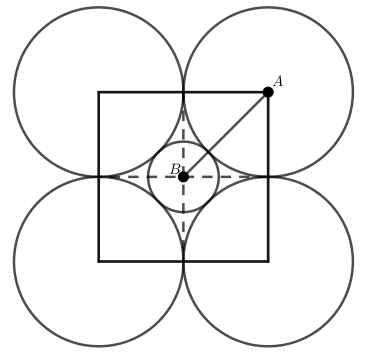
\includegraphics[width=0.5\textwidth]{images/diagonal 2d.png}
    \caption{\label{fig:2d diagonal}Unit 2-cube diagonal length determined using Extended Pythagorean Theorem}
\end{figure}

\noindent Hence, we can subtract the unit circle radius to obtain the radius of the two-dimensional IK-Sphere: $$r_2 = \sqrt{1^2+1^2}-1.$$  %Then, dividing by 2, we get the radius of an IK-Sphere in two-dimensions: $$r_2=\frac{\sqrt{1^2+1^2}-2}{2}.$$ 

Similarly, for a three-dimensional IK-Sphere, the length of the diagonal is the square root of the sum of three sides of of an octant ($\frac{1}{8}$ of a cube) of the $n$-cube at a vertex (see Figure \ref{fig:3d diagonal}). From there, the process is the same and we subtract the unit sphere. Thus, we have an inscribed sphere radius $r_3$ of: 

\begin{equation*}
    r_3=\sqrt{1^2+1^2+1^2}-1.
\end{equation*}

\begin{figure}[H]
    \centering
    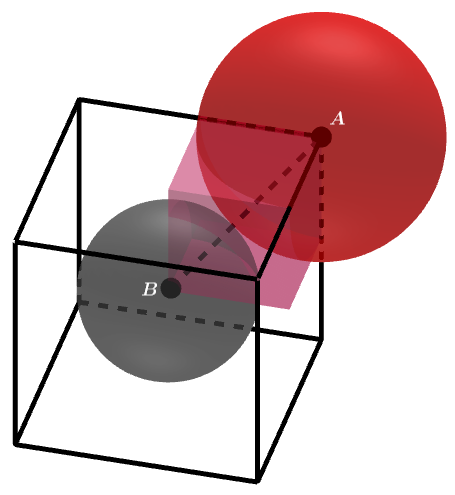
\includegraphics[width=0.6\textwidth]{images/3d diagonal.png}
    \caption{\label{fig:3d diagonal}Unit 3-cube diagonal length determined using Extended Pythagorean Theorem}
\end{figure}

\begin{corollary}[To the Extended Pythagorean Theorem for $n$-Cubes] The diagonal $c$ of a unit $n$-cube is given by
\begin{equation} \label{ncube diagonal}
    c = \sqrt{n}
\end{equation}
\end{corollary}
\begin{proof}
    Substituting $a=1$ into the extended Pythagorean Theorem (see Equation \ref{extendedpythag}), we have
    \begin{align*}
        c^2 &= \sum_{i}^{n}1_i^2\\
        &=n\\
        \therefore c &= \sqrt{n}.
    \end{align*}
\end{proof}

If the diagonal of a unit $n$-cube is given by $\sqrt{n}$ (see Equation \ref{ncube diagonal}), the IK-Sphere radius can be generalised across all $n$-dimensions by subtracting the unit sphere radius as follows:
\begin{equation}\label{radius of ik sphere}
    r_n = \sqrt{n}-1
\end{equation}

\noindent
We may now proceed to the final step of proving that the radius of an IK-Sphere increases without bound.

\begin{theorem}\label{theorem:radius of IK-Sphere}
As the dimension $n$ tends to infinity, the radius $r_n$ of the inscribed sphere also tends to infinity.
\end{theorem}
\begin{proof}
Take the limit as $n$ approaches infinity of the expression for $r_n$ in terms of $n$ (See Equation \ref{radius of ik sphere}) and apply the limit difference rule. 

\noindent
Limit Difference Rule: $\lim_{a\to b} x-y =  \lim_{a\to b}x - \lim_{a\to b}y$.

\noindent
Thus, we have
\begin{align*}
    \lim_{n\to\infty} \sqrt{n}-1 &= \lim_{n\to\infty} \sqrt{n} - \lim_{n\to\infty} \sqrt{1}\\
    &=\infty - 1\\
    &=\infty.
\end{align*}
$\therefore$ the radius of an IK-Sphere diverges to infinity as dimension $n$ increases.\\
\end{proof}

Graphically (see Figure \ref{fig:radius increases graph}), we may observe the same result with less rigour. The domain has been restricted to $n\geq3$ as $n=3$ was the base case for the Extended Pythagorean Theorem for an $n$-Cube (see Lemma \ref{lemma:extend pythag}). Below $n=1$ we obtain negative values for $r_n$ which can accordingly be considered an undefined region. Investigation into fractional dimensions (such as those observed in fractals) could reveal a reason, however, that is currently beyond the scope of this essay.
%Here begins the 2D plot
\begin{figure}[H]
    \centering
    \begin{tikzpicture}
        \begin{axis}[
            axis lines = left,
            xlabel = \(n\),
            ylabel = {\(r_n\)},
        ]
        %Below the red parabola is defined
        \addplot [
            domain=3:100, 
            samples=100, 
            color=red,
        ]
        {sqrt(x)-1};
        \addlegendentry{\(\sqrt{n}-1\)}
        %Here the blue parabola is defined
        \end{axis}
    \end{tikzpicture}
    \caption{Radius increases without bound as dimensionality increases.}
    \label{fig:radius increases graph}
\end{figure}
%Here ends the 2D plot






\section{Verification of the IK-Sphere Intersection in Four Dimensions}\label{section:verify intersection}
The radius of an IK-Sphere has now been proven to increase without bound. As such, one may infer that the IK-Sphere bursts outside of its bounding box as dimensionality increases, implying that there exist intersection points between the IK-Sphere and its `bounding' $n$-cube at higher dimensions. In fact, upon inspection, one may observe that at $n=4$ dimensions, $$r_4=\sqrt{4}-1=1.$$ The IK-Sphere just touches the sides of its bounding 4-cube with side length 2 units (!). Here, intuition takes hold once again. One may assume there exists a solvable intersection point in the center of a single face of the 4-cube with the IK-Sphere. However, another possibility arises in which higher dimensional intersections may operate differently and the IK-Sphere may still exist within its bounding $n$-cube as we originally assumed. We can verify the existence, or lack thereof, of an intersection point to decide which of these possibilities is true in higher dimensions.

To solve for the intersection point, we would need two equations in 4 coordinate variables $(x, y, z, w)$: one for the 4-cube and one for the 4-sphere. From the definition of an $n$-sphere (see Definition \ref{def:n-sphere}) the following equation can be constructed:
\begin{lemma}
In four-dimensional space with coordinates $(x, y, z, w)$, a unit 4-sphere can be defined as
\begin{equation}\label{eq:unit 4-sphere}
    x^2+y^2+z^2+w^2=1.
\end{equation}
where $(x, y, z, w)$ is a point on the 4-sphere.
\end{lemma}
\begin{proof}
    This is a simple proof using vectors. Consider the vector $\Vec{\mathbf{r}}$ originating from the center of the 4-sphere. For the span of this vector to be a unit 4-sphere, the magnitude of $\Vec{\mathbf{r}}$ must equal 1. In notation, this is $$\lVert\Vec{\mathbf{r}}\rVert = 1.$$
    Expanding $\lVert\Vec{\mathbf{r}}\rVert$ then squaring both sides, we can obtain the required result:
    \begin{align*}
        \sqrt{x^2+y^2+z^2+w^2}&=1\\
        \therefore x^2+y^2+z^2+w^2&=1
    \end{align*}
\end{proof}

However, an explicit equation for the entire 4-cube is not readily available. As such, we will use a single face of the 4-cube, or rather, a plane in 4-dimensions with restrictions $0\leq x, y, z, w \leq 2$. Let this plane be denoted by $\Pi$.
\begin{definition}[$n$-Plane]
    An $(n-1)$-dimensional space extending to infinity in all $n-1$ dimensions embedded in $n$-dimensional space. Examples include: a line in $\mathbb{R}^2$, a plane in $\mathbb{R}^3$, $\mathbb{R}^3$ space embedded in $\mathbb{R}^4$.
\end{definition}
\begin{lemma}
A 4-plane can be represented by the equation \begin{equation}\label{eq:4-plane}
    ax+by+cz+dw=k
\end{equation}
where $a, b, c, d, k$ are constants and $(x, y, z, w)$ is a point on $\Pi$. 
\end{lemma}
\begin{proof}
    Let the vector $\Vec{\mathbf{r}}$ denote a position vector $\langle x, y, z, w\rangle$ from the origin to any point on $\Pi$, $\Vec{\mathbf{a}}$ be a position vector to a fixed point $\langle x_0, y_0, z_0, w_0\rangle$ contained within $\Pi$, $\Vec{\mathbf{n}}$ be a normal direction vector $\langle a, b, c, d\rangle$ to $\Pi$, and $\Vec{\mathbf{v}}$ be the direction vector $\langle x-x_0, y-y_0, z-z_0, w-w_0\rangle$ contained within $\Pi$. In $\mathbb{R}^3$ this is represented in Figure \ref{fig:plane equation proof setup}.
    \begin{figure}[H]
        \centering
        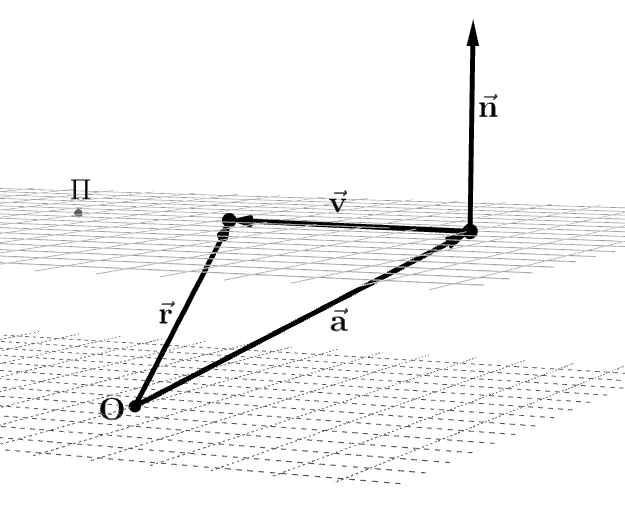
\includegraphics[width=0.8\textwidth]{images/vector equation of plane.png}
        \caption{A plane containing a point and vector, and a normal vector to $\Pi$.}
        \label{fig:plane equation proof setup}
    \end{figure}
    
    \noindent
    The vector $\Vec{\mathbf{v}}$ is in $\Pi$ if and only if $$\Vec{\mathbf{v}} \cdot \Vec{\mathbf{n}} = 0.$$ Expanding $\Vec{\mathbf{v}}$ and $\Vec{\mathbf{n}}$ we have $$\langle x-x_0, y-y_0, z-z_0, w-w_0\rangle \cdot \langle a, b, c, d\rangle = 0.$$
    
    \noindent
    Then, by calculating the dot product and rearranging, we can obtain the form $ax+by+cz+dw=k$:
    \begin{align*}
        a(x-x_0)+b(y-y_0)+c(z-z_0)+d(w-w_0) &= 0\\
        ax+by+cz+dw-ax_0-by_0-cz_0-dw_0 &= 0\\
        ax+by+cz+dw = ax_0+by_0+cz_0+dw_0
    \end{align*}
    Letting $ax_0+by_0+cz_0+dw_0=k$ gives
    \begin{align*}
        ax+by+cz+dw = k
    \end{align*}
    as required.
\end{proof}

We now have two equations for a 4-plane (see Equation \ref{eq:4-plane}) and a unit $4$-sphere (see Equation \ref{eq:unit 4-sphere}):
\begin{quote}
    4-plane:$$ax+by+cz+dw=k;$$
    unit 4-sphere: $$x^2+y^2+z^2+w^2=1.$$
\end{quote}

\noindent
However, before solving for an intersection in four variables, we need to find the constants $a, b, c, d$, and $k$. From the definition of the $n$-cube (see Definition \ref{def:n-cube}), we can deduce that a face of the 4-cube will lie on one of the $x, y, z, w$ axes. Let us make this the $w$ axis. Thus, a point on $\Pi$ will be of the form $(x, y, z, 0)$ where $0\leq x, y, z \leq 2$ so as to restrict it to be a face of the bounding 4-cube. We can now simplify the equation of $\Pi$ as long as we maintain that $x, y$, and $z$ satisfy $0\leq x, y, z \leq 2$. The equation of $\Pi$, hence,  simplifies to
\begin{equation}\label{eq:cube face}
    w=0.
\end{equation}

We then determine the specific equation of the IK-sphere centered at $(1, 1, 1, 1)$ in the middle of the 4-cube. When the vector $\Vec{\mathbf{r}}$ from the center of the IK-sphere has a magnitude $\lVert\Vec{\mathbf{r}}\rVert=0$, its components $\langle x, y, z, w\rangle=\langle 1, 1, 1, 1\rangle$ because they must be the center coordinates of the 4-sphere (vector with magnitude of zero is a point). Thus, we obtain the equation for our IK-sphere centered at $(1, 1, 1, 1)$:
\begin{equation}\label{eq:IK 4 sphere centered at 1}
    (x-1)^2+(y-1)^2+(z-1)^2+(w-1)^2=1
\end{equation}

The coordinate(s) of intersection between the plane and IK-sphere where $0\leq x, y, z \leq 2$ can now be solved for. Substituting $w=0$ from the equation of the plane $\Pi$ (see Equation \ref{eq:cube face}) into the equation of the IK-sphere (see Equation \ref{eq:IK 4 sphere centered at 1}) and simplifying, 
\begin{align*}
    (x-1)^2+(y-1)^2+(z-1)^2+1&=1\\
    (x-1)^2+(y-1)^2+(z-1)^2&=0,
\end{align*}
we can solve for $x, y$, and $z$ because for any arbitrary value $\alpha$,
\begin{align*}
    \forall  \alpha \in \mathbb{R}, (\alpha-1)^2 \geq 0 \implies \forall \alpha \ni \alpha \geq 0, \left( (x-1), (y-1), (z-1)\right) = 0.\\
\end{align*}
\begin{align*}
    \therefore (x, y, z)=(1, 1, 1). 
\end{align*}
Thus, the intersection between the IK-sphere and its bounding 4-cube's $w=0$ face occurs at $(1,1,1,0)$ and there is only one solution. This is directly in the center of the face as expected. In response to the research question, \researchquestion it has been verified that an IK-Sphere does share a coordinate with its bounding $n$-cube at $n=4$ dimensions. Additionally, we provided algebraic reasoning for the radius of an IK-Sphere tending to infinity by proving that the limit of the expression for the radius of an IK-Sphere in terms of $n$ approaches infinity as $n \to \infty$. However, a more visual high dimensional intuition can be provided through geometric reasoning as detailed in the following chapter.

% four different equations:  
% \begin{equation*}
%     \systeme*{
%     a(1)+b(0)+c(0)+d(0)=k,
%     a(0)+b(1)+c(0)+d(0)=k,
%     a(0)+b(0)+c(1)+d(0)=k,
%     a(0)+b(0)+c(0)+d(1)=k.
%     }
% \end{equation*}
% \noindent
% However, we must determine the constant $k$ before this system of equations is solvable. 
% \begin{lemma}
%     The constant $k$ in the equation for plane $\Pi$ can be any $k > 0$, $k \in \mathbb{R}$.
% \end{lemma}
% \begin{proof}
%     We know from the equation of a plane $\Vec{\mathbf{r}} \cdot \Vec{\mathbf{n}} = \Vec{\mathbf{a}} \cdot \Vec{\mathbf{n}}$ that \(k=\Vec{\mathbf{a}} \cdot\Vec{\mathbf{n}}\) where $\Vec{\mathbf{r}}$ is the position vector to any point on $\Pi$, $\Vec{\mathbf{n}}$ is the normal vector $\langle a, b, c, d \rangle$ to $\Pi$ and $\Vec{\mathbf{a}}$ is a fixed point on $\Pi$.
    
%     \noindent
%     We can set $\Vec{\mathbf{a}} = \langle 1, 1, 1, 0 \rangle$ because it satisfies $0\leq x, y, z \leq 2$ for it to be within $\Pi$. Consequently, if $\Vec{\mathbf{a}} = \langle 1, 1, 1, 0 \rangle$,
%     \begin{align*}
%         k &= \Vec{\mathbf{a}} \cdot\Vec{\mathbf{n}}\\
%           &= \langle 1, 1, 1, 0\rangle \cdot \langle a, b, c, d\rangle\\
%           &= a + b + c
%     \end{align*}
%     The magnitude of $\Vec{\mathbf{n}}$ can be any $ \lVert\Vec{\mathbf{n}}\rVert > 0$, $\lVert\Vec{\mathbf{n}}\rVert\in \mathbb{R}$ which implies that $a+b+c+d > 0$ and $k = a+b+c+d$ so $k>0$.
% \end{proof}

% Therefore, we set $k=1$ giving the following system of equations:
% \begin{equation*}
%     \systeme*{
%     a(1)+b(0)+c(0)+d(0)=1,
%     a(0)+b(1)+c(0)+d(0)=1,
%     a(0)+b(0)+c(1)+d(0)=1,
%     a(0)+b(0)+c(0)+d(1)=1.
%     }
% \end{equation*}
% \noindent
% This system of equations is equivalent to the augmented matrix which, in reduced row echelon form, evaluates to
% \begin{align*}
%     \begin{amatrix}{4}
%         1 & 0 & 0 & 0 & 1 \\  
%         0 & 1 & 0 & 0 & 1 \\
%         0 & 0 & 1 & 0 & 1 \\
%         0 & 0 & 0 & 0 & 1
%     \end{amatrix}
% \end{align*}
% However, such a matrix has no solutions (observe last row



